%%%%%%%%%%%%%%%%%%%%%%%%%%%%%%%%%%%%%%%%%
% Short Sectioned Assignment
% LaTeX Template
% Version 1.0 (5/5/12)
%
% This template has been downloaded from:
% http://www.LaTeXTemplates.com
%
% Original author:
% Frits Wenneker (http://www.howtotex.com)
%
% License:
% CC BY-NC-SA 3.0 (http://creativecommons.org/licenses/by-nc-sa/3.0/)
%
%%%%%%%%%%%%%%%%%%%%%%%%%%%%%%%%%%%%%%%%%

%----------------------------------------------------------------------------------------
%	PACKAGES AND OTHER DOCUMENT CONFIGURATIONS
%----------------------------------------------------------------------------------------

\documentclass[paper=a4, fontsize=11pt]{scrartcl} % A4 paper and 11pt font size

\usepackage[utf8]{inputenc}
%\usepackage[T1]{fontenc} % Use 8-bit encoding that has 256 glyphs
\usepackage{fourier} % Use the Adobe Utopia font for the document - comment this line to return to the LaTeX default
\usepackage[english]{babel} % English language/hyphenation
\usepackage{amsmath,amsfonts,amsthm} % Math packages

\usepackage{nameref}
\usepackage{graphicx} % Required to insert images
%\usepackage{lipsum} % Used for inserting dummy 'Lorem ipsum' text into the template

\usepackage{sectsty} % Allows customizing section commands
\allsectionsfont{\centering \normalfont\scshape} % Make all sections centered, the default font and small caps

\usepackage{fancyhdr} % Custom headers and footers
\pagestyle{fancyplain} % Makes all pages in the document conform to the custom headers and footers
\fancyhead{} % No page header - if you want one, create it in the same way as the footers below
\fancyfoot[L]{} % Empty left footer
\fancyfoot[C]{} % Empty center footer
\fancyfoot[R]{\thepage} % Page numbering for right footer
\renewcommand{\headrulewidth}{0pt} % Remove header underlines
\renewcommand{\footrulewidth}{0pt} % Remove footer underlines
\setlength{\headheight}{13.6pt} % Customize the height of the header

%\numberwithin{equation}{section} % Number equations within sections (i.e. 1.1, 1.2, 2.1, 2.2 instead of 1, 2, 3, 4)
%\numberwithin{figure}{section} % Number figures within sections (i.e. 1.1, 1.2, 2.1, 2.2 instead of 1, 2, 3, 4)
%\numberwithin{table}{section} % Number tables within sections (i.e. 1.1, 1.2, 2.1, 2.2 instead of 1, 2, 3, 4)

\setlength\parindent{0pt} % Removes all indentation from paragraphs - comment this line for an assignment with lots of text

%----------------------------------------------------------------------------------------
%	TITLE SECTION
%----------------------------------------------------------------------------------------

\newcommand{\horrule}[1]{\rule{\linewidth}{#1}} % Create horizontal rule command with 1 argument of height

\title{	
\normalfont \normalsize 
\textsc{Università della Svizzera Italiana, Faculty of Informatics} \\ [25pt] % Your university, school and/or department name(s)
\horrule{0.5pt} \\[0.4cm] % Thin top horizontal rule
\huge Localisation \\ % The assignment title
\horrule{2pt} \\[0.5cm] % Thick bottom horizontal rule
}

\author{Simon Maurer} % Your name

\date{\normalsize\today} % Today's date or a custom date

\begin{document}

\maketitle % Print the title

%----------------------------------------------------------------------------------------
%	PROBLEM 1
%----------------------------------------------------------------------------------------

\section{Assignment 5.1}
All implementations have been tested on Octave
\footnote{https://www.gnu.org/software/octave/} version 3.6.4.

The following probabilities have been used
\begin{itemize}
    \item $ P(a|b) = 0.8 $
    \item $ P(\bar{a}|b) = 0.2 $
    \item $ P(a|\bar{b}) = 0.4 $
    \item $ P(\bar{a}|\bar{b}) = 0.6 $
\end{itemize}
with the events
\begin{itemize}
    \item Event $ a $: see landmark
    \item Event $ \bar{a} $: see no landmark
    \item Event $ b $: is on landmark
    \item Event $ \bar{b} $: is not on landmark
\end{itemize}

\subsection{Bayes Localization}
By using the discrete Bayes filter the probabilities for the robot to be at
a position at each instant in time are computed. The implemented algorithm can
be found in the file \emph{ex05\_bayesian.m}.  The results are represented in
Figure \ref{fig:bayes}. With the given movements, sensor results and
probabilities, it is most probable that the robot ends on position 7 (hence
started on position 0).

\begin{figure}[h]
    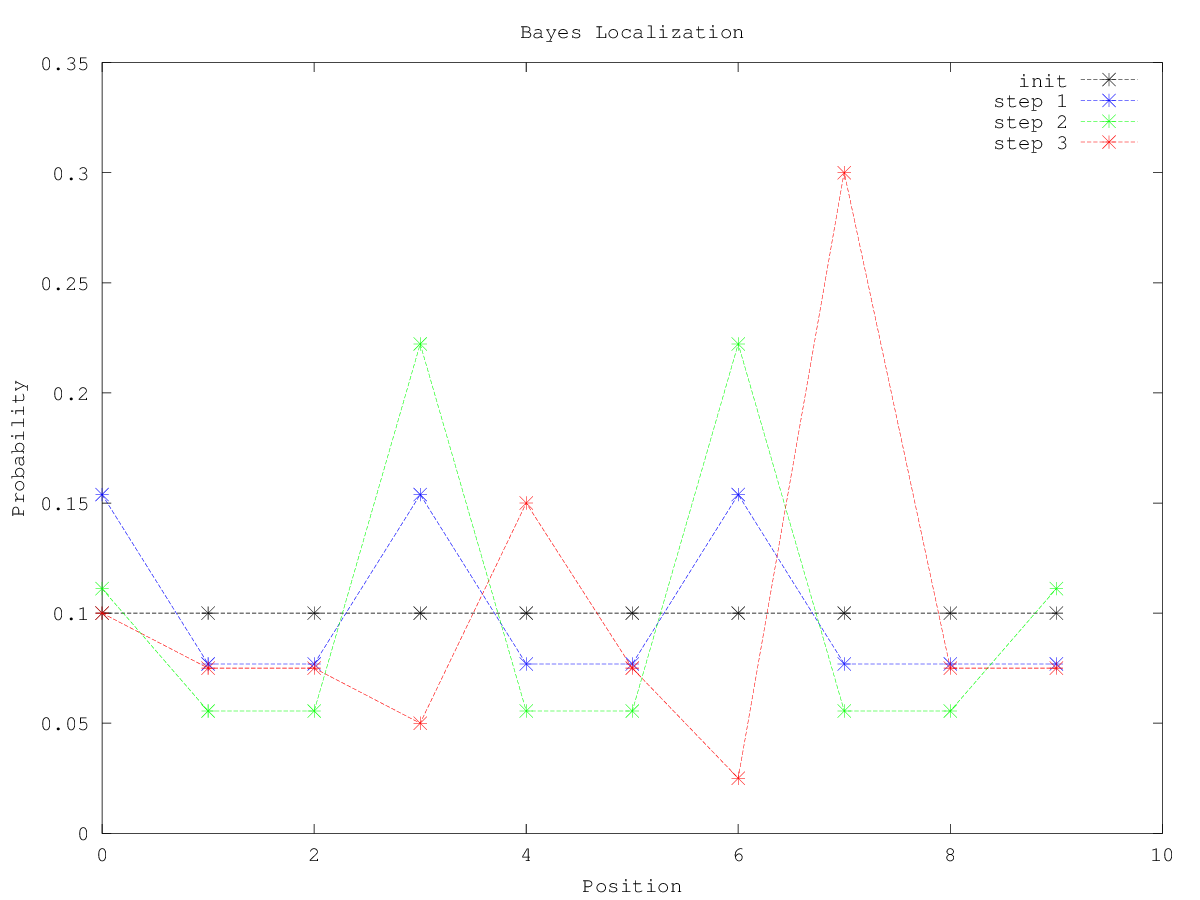
\includegraphics[width=1\columnwidth]{ex05_graph1}
    \caption{Probabilities of the position of the robot after each time step}
    \label{fig:bayes}
\end{figure}

\subsection{Monte Carlo Localization}
Using the particle filter algorithm, again the probabilities for the robot to
be at a position for each time step are computed. The file
\emph{ex05\_particle.m} explains the implementation. The graph on the top of
figure \ref{fig:particle} shows the results assuming a perfect movement and the
graph on the bottom shows the results assuming, the robot only moves with
a probability of $ 80\% $. In both cases 1000 particles have been used. By
decreasing the number of particles, the results are more random (i.e. by
running the experiment multiple times, the results differ from one to another).
The smaller the number of particles the worse the results. In case of 10
particles, the result is not usable. Also here it is most probable, that the
robot ends on position 7 (starts on position 0). In case of the movement error,
the probability of ending at position 7 is a bit lower than in the case of
perfect movement.

\begin{figure}[h]
    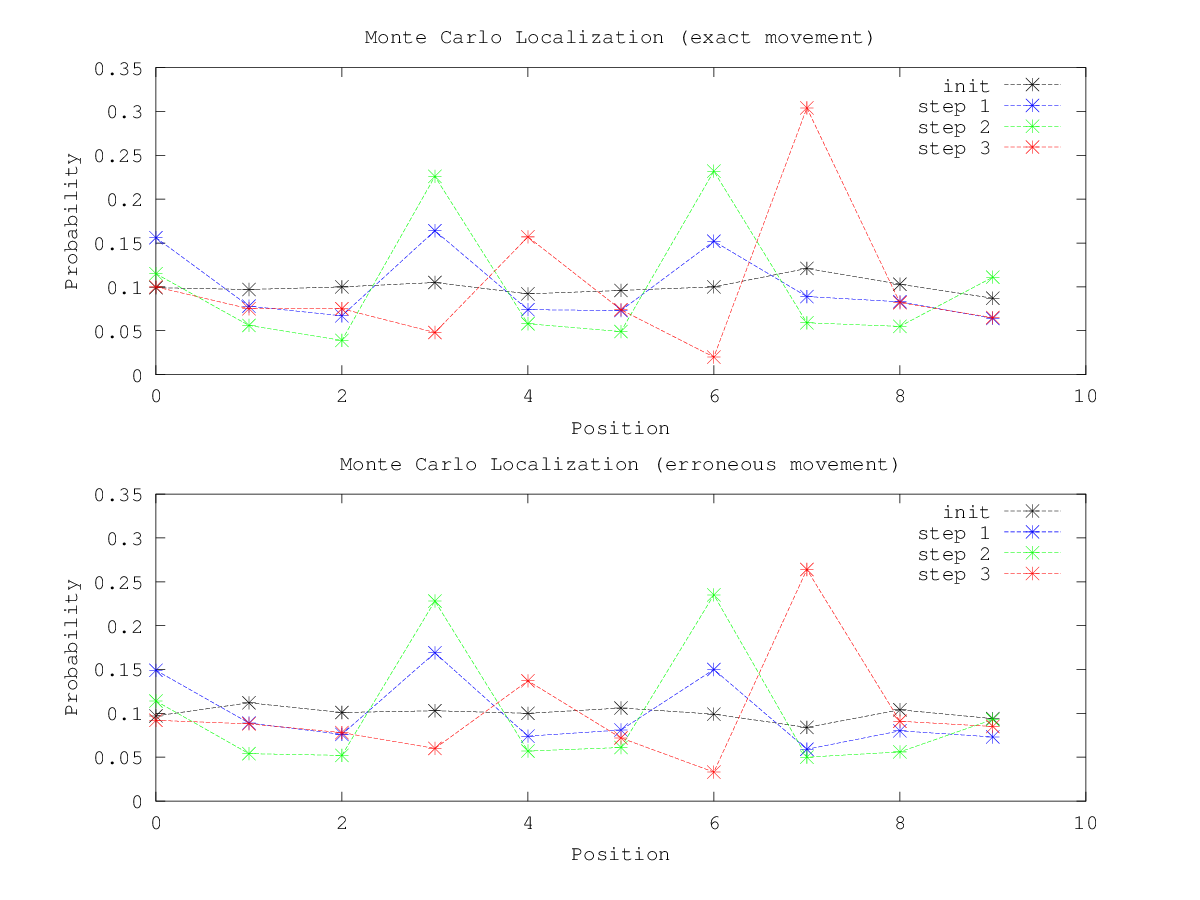
\includegraphics[width=1\columnwidth]{ex05_graph2}
    \caption{Probabilities of the position of the robot after each time step.
        Top: perfect movement, bottom: erroneous movement}
    \label{fig:particle}
\end{figure}
\end{document}
